% Chapter Template

\chapter{Elderly care demo} % Main chapter title

\label{Chapter7} % Change X to a consecutive number; for referencing this chapter elsewhere, use \ref{ChapterX}

%----------------------------------------------------------------------------------------
%	SECTION 1
%----------------------------------------------------------------------------------------
The chapter will first address the issue being solved, then the methodology will be presented and finally the results will be presented.
Elderly care has been addressed by many EU funded research projects since aging population is one of the issues the union is facing. 
There are many solutions for this problem, from invasive such as wearables, sound sensors, IR occupancy detector, etc. 
Few papers tried to solve this issue using non-invasive using previously mentioned NILM algorithms. 
In this case no additional meters need to be installed, since per-appliance usage can be disagreed from main meter time-series data. 
While this is practical from new equipment side, it is a bit less from accuracy side for larger buildings. 
There is a middle way between invasive and non-invasive ways. 
It is possible to set up sub-meters behind each appliance, and indirectly observe the usage pattern for this elder person. 
This is better since the elder does not need to wear the device, but it is a bit slower in detecting the accident. 

\section{Goal}

The chapter will focus on building the elderly care system that will use users periodic usage pattern to detect an anomaly.
The anomaly could be anything from a fall, stroke or altered usage pattern due to dementia. 
Algorithm will be designed based on load profile from previous chapter \ref{fig:PHPA}.
Figure shows, that first thing in the morning used are kettle and toaster, and with delay of one hour, microwave and TV. 
If none of these appliances are used within that hour, then that hour is considered anomalous.
This means that the algorithm will be able to detect the anomaly within 1 hour of accident.

\section{Methodology}

\subsection{Building anomaly detection algorithm}

Next section will present steps taken wile designing this algorithm.

\subsubsection{Step one}
To detect the anomalies one first needs to build a daily activation profile for each appliance, such as the one previously mentioned \ref{fig:PHPA}.
In this specific case we will be using 2h buckets, yielding total of 12 buckets. 

\subsubsection{Step two}
Second step is to ignore appliances that are always on by calculating the standard deviation of activations for each bucket. 
The activations are normalised between 0 and 1. 
This step is important so that appliances that are always on, such as fridge or freezer get ignored. 
These appliances are detected based on width of their activations normal distribution. 
Where periodic (hourly basis) appliances should have narrow distributions, the more dynamic should have wider distributions.
This can be seen on examples from building 2.

\begin{figure}[H]
    \centering
    \begin{tikzpicture}
        \coordinate (s) at (0,0);
        \foreach \num in {866, 842, 810, 772, 868, 854, 859, 854, 864, 887, 889, 883}{
        \node[minimum size=6mm, draw, rectangle] at (s) {\num};
        \coordinate (s) at ($(s) + (1,0)$);
        }
    \end{tikzpicture}
    \caption{Daily activations for fridge $\sigma$ = 0.036}
    \label{arr:fridge_acts}
\end{figure}

\begin{figure}[H]
    \centering
    \begin{tikzpicture}
        \coordinate (s) at (0,0);
        \foreach \num in {86, 77, 75, 74, 100, 118, 113, 127, 168, 202, 171, 121}{
        \node[minimum size=6mm, draw, rectangle] at (s) {\num};
        \coordinate (s) at ($(s) + (1,0)$);
        }
    \end{tikzpicture}
    \caption{Daily activations for audio system $\sigma$ = 0.2}
    \label{arr:as_acts}
\end{figure}

\begin{figure}[H]
    \centering
    \begin{tikzpicture}
        \coordinate (s) at (0,0);
        \foreach \num in {9, 4, 4, 3, 212, 122, 85, 80, 102, 260, 134, 48}{
        \node[minimum size=6mm, draw, rectangle] at (s) {\num};
        \coordinate (s) at ($(s) + (1,0)$);
        }
    \end{tikzpicture}
    \caption{Daily activations for microwave $\sigma$ = 0.3}
    \label{arr:microwave_acts}
\end{figure}

Based results from all appliances a threshold of $\sigma$ = 0.1 was set.
This method will also get rid of appliances that are always on due to their specific nature such as server computer, 
or are rarely used. 

\subsubsection{Third step}

Next, appliances that trigger together must be grouped. 
This means we must find part of the day that they are operating in.
Due to filter in previous step, we are left with appliaces whos usage variates trough the day. 
Some appliances are on even when user is not necesariliy using them, this can be seen on figure \ref{arr:as_acts}.
One out of many ways to do this is to normalize the activations, this yields a metric that tells us the probability of that appliance being turned on compared to the rest of the day. 
If we do this for same appliances as above the result is following: 

\begin{figure}[H]
    \centering
    \begin{tikzpicture}
        \coordinate (s) at (0,0);
        \foreach \num in {0.43, 0.38, 0.37, 0.37, 0.5 , 0.58, 0.56, 0.63, 0.83, 1. , 0.85,
        0.6}{
        \node[minimum size=6mm, draw, rectangle] at (s) {\num};
        \coordinate (s) at ($(s) + (1,0)$);
        }
    \end{tikzpicture}
    \caption{Daily activations for audio system $\sigma$ = 0.2}
    \label{arr:as_acts_norm}
\end{figure}

\begin{figure}[H]
    \centering
    \begin{tikzpicture}
        \coordinate (s) at (0,0);
        \foreach \num in {0.03, 0.02, 0.02, 0.01, 0.82, 0.47, 0.33, 0.31, 0.39, 1.  , 0.52,
        0.18}{
        \node[minimum size=6mm, draw, rectangle] at (s) {\num};
        \coordinate (s) at ($(s) + (1,0)$);
        }
    \end{tikzpicture}
    \caption{Daily activations for microwave $\sigma$ = 0.3}
    \label{arr:microwave_acts_norm}
\end{figure}

Finnaly a suitable threshold must be selected.
The treshold of .5 was selected, which yields the folowing vectors:

\begin{figure}[H]
    \centering
    \begin{tikzpicture}
        \coordinate (s) at (0,0);
        \foreach \num in {0, 0, 0, 0, 0 , 1, 1, 1, 1, 1 , 1, 1}{
        \node[minimum size=6mm, draw, rectangle] at (s) {\num};
        \coordinate (s) at ($(s) + (1,0)$);
        }
    \end{tikzpicture}
    \caption{Daily activations for audio system}
    \label{arr:as_acts_vec}
\end{figure}

\begin{figure}[H]
    \centering
    \begin{tikzpicture}
        \coordinate (s) at (0,0);
        \foreach \num in {0, 0, 0, 0, 1, 0, 0, 0, 0, 1, 1, 0}{
        \node[minimum size=6mm, draw, rectangle] at (s) {\num};
        \coordinate (s) at ($(s) + (1,0)$);
        }
    \end{tikzpicture}
    \caption{Daily activations for microwave with one usage peak in the morning and the other in the evening}
    \label{arr:microwave_acts_vec}
\end{figure}

The vectors show us that microwave has two usage peaks, where audio system can be used anytime through the day.
It is possible to do this over all appliances, which results a 2D matrix. 
Using this matrix we can build rules witch which appliances are being used together
The figure \ref{arr:act_mat} uses rows for appliances and columns for buckets.  
If we use terminology from image processing the matrix \ref{arr:act_mat} is essentially highly saturated load profile \ref{fig:PHPA},
that can be easily processed by computer algorithms due to binary encoding. 

\begin{figure}[H]
    \centering
    \begin{tikzpicture}
        \coordinate (s) at (0,6);
        \foreach \num in {0, 0, 0, 0, 0, 1, 1, 1, 1, 1, 1, 1}{
        \node[minimum size=6mm, draw, rectangle] at (s) {\num};
        \coordinate (s) at ($(s) + (1,0)$);
        }
        \coordinate (s) at (0,5);
        \foreach \num in {0, 0, 0, 0, 0, 0, 0, 0, 0, 1, 1, 1}{
        \node[minimum size=6mm, draw, rectangle] at (s) {\num};
        \coordinate (s) at ($(s) + (1,0)$);
        }
        \coordinate (s) at (0,4);
        \foreach \num in {0, 0, 0, 0, 0, 0, 0, 0, 1, 1, 0, 0}{
        \node[minimum size=6mm, draw, rectangle] at (s) {\num};
        \coordinate (s) at ($(s) + (1,0)$);
        }
        \coordinate (s) at (0,3);
        \foreach \num in {0, 0, 0, 0, 1, 0, 0, 1, 1, 1, 1, 0}{
        \node[minimum size=6mm, draw, rectangle] at (s) {\num};
        \coordinate (s) at ($(s) + (1,0)$);
        }
        \coordinate (s) at (0,2);
        \foreach \num in {0, 0, 0, 0, 1, 1, 0, 0, 1, 0, 0, 0}{
        \node[minimum size=6mm, draw, rectangle] at (s) {\num};
        \coordinate (s) at ($(s) + (1,0)$);
        }
        \coordinate (s) at (0,1);
        \foreach \num in {0, 0, 0, 0, 1, 0, 1, 0, 0, 0, 1, 0}{
        \node[minimum size=6mm, draw, rectangle] at (s) {\num};
        \coordinate (s) at ($(s) + (1,0)$);
        }
        \coordinate (s) at (0,0);
        \foreach \num in {0, 0, 0, 0, 0, 1, 1, 1, 1, 1, 0, 0}{
        \node[minimum size=6mm, draw, rectangle] at (s) {\num};
        \coordinate (s) at ($(s) + (1,0)$);
        }
    \end{tikzpicture}
    \caption{Activation matrix}
    \label{arr:act_mat}
\end{figure}


\subsubsection{Step four}

Using the matrix \ref{arr:act_mat} we can write an algorithm that will use current activations 
and compare it the matrix. For an example if we have the live data for the fifth bucket, that is 
data from 8 to 10 o clock. 
What needs to be done is to use the fifth column and muliply to the current activations.
Then anomaliy is detected based on a rule, if sum of multiplied array equals to zero the 
bucket is considered anomalous. The higher the sum, the more sure the algorithm is that the
bucket is normal. 

\begin{figure}[H]
    \centering
    \begin{tikzpicture}
        \coordinate (s) at (0,5);
        \foreach \num in {0, 0, 0, 0, 0, 0, 0, 1, 1, 1, 1, 0}{
        \node[minimum size=6mm, draw, rectangle] at (s) {\num};
        \coordinate (s) at ($(s) + (1,0)$);
        }
        
        \node at (5.5,4) {X};
        \coordinate (s) at (0,3);
        \foreach \num in {1, 0, 0, 0, 0, 0, 0, 1, 0, 0, 1, 0}{
        \node[minimum size=6mm, draw, rectangle] at (s) {\num};
        \coordinate (s) at ($(s) + (1,0)$);
        }
        \node at (5.5,2){=};
        \coordinate (s) at (0,1);
        \foreach \num in {0, 0, 0, 0, 0, 0, 0, 1, 0, 0, 1, 0}{
        \node[minimum size=6mm, draw, rectangle] at (s) {\num};
        \coordinate (s) at ($(s) + (1,0)$);
        }
        \node at (5.5,0){SUM = 2 - > not an anomaly };
    \end{tikzpicture}
    \caption{The evaluation of new bucket compared to matrix. Example is for fifth bucket or fifth row from the matrix}
    %\label{arr:microwave_acts_vec}
\end{figure}

This process is done for all samples, where we count normal and anomolus samples for each bucket
Important thing to note here is that we are evaluating on the samples that the profile was built on.

\begin{figure}[H]
    \centering
    \begin{tikzpicture}
        \coordinate (s) at (0,0);
        \foreach \num in {472, 469, 468, 466, 57, 153, 288, 187, 123, 84, 75, 281}{
        \node[minimum size=6mm, draw, rectangle] at (s) {\num};
        \coordinate (s) at ($(s) + (1,0)$);
        }
    \end{tikzpicture}
    \caption{Agregated anomalies for each bucket}
    \label{arr:agg_anom}
\end{figure}

\begin{figure}[H]
    \centering
    \begin{tikzpicture}
        \coordinate (s) at (0,0);
        \foreach \num in {0, 0, 0, 0, 409, 312, 181, 280, 342, 384, 394, 188}{
        \node[minimum size=6mm, draw, rectangle] at (s) {\num};
        \coordinate (s) at ($(s) + (1,0)$);
        }
    \end{tikzpicture}
    \caption{Agregated normal samples for each bucket}
    \label{arr:agg_norm}
\end{figure}

Next step is to combine these two arrays, so that we calcuate the percentae of anomalous samples 
for each bucket with an equation

\begin{equation}
    a / (a + n) 
\end{equation}

Where a is a number of anomolus samples and n is a number of normal samples.

\begin{figure}[H]
    \centering
    \begin{tikzpicture}
        \coordinate (s) at (0,0);
        \foreach \num in {1.0, 1.0, 1.0, 1.0, 0.12, 0.3, 0.61, 0.4, 0.26, 0.18, 0.16, 0.6}{
        \node[minimum size=6mm, draw, rectangle] at (s) {\num};
        \coordinate (s) at ($(s) + (1,0)$);
        }
    \end{tikzpicture}
    \caption{Agregated anomalies for each bucket}
    \label{arr:anom_ratio}
\end{figure}

In other words the \ref{arr:anom_ratio} tells us how persistent is the users routine in each bucket or
part of the day. The lower the ratio the higher the routine. Since routine is detected based on usage
of appliances it cannot be picked up during the night. It is possible to see that routine is quite high 
during morning and evening hours. The anomaly detection algorithm will work best when ratio above is low.
Good trait of elder is that their routine is quite high even during the day, which means that
the anomaly detection will function better and throughout the day.

One more thing to do is to ignore the parts of the day when user has no routine, by using
the array \ref{arr:anom_ratio} and setting a threshold of 0.3. A threshold of 0.5 would mean
that every other day could be a false positive anomaly. Setting the rate at 0.3 reduces that 
to every third day. But here compromises must be made, the lower the threshold the more accurate
the algorithm will be, but it also means that it will be less sensitive. 
In our case there is not much harm in false positives detections, since the caregiver can call
the elder to check if it is okay.  

\begin{figure}[H]
    \centering
    \begin{tikzpicture}
        \coordinate (s) at (0,0);
        \foreach \num in {0, 0, 0, 0, 1, 1, 0, 0, 1, 1, 1, 0}{
        %\foreach \num in {1.0, 1.0, 1.0, 1.0, 0.12, 0.3, 0.61, 0.4, 0.26, 0.18, 0.16, 0.6}{
        \node[minimum size=6mm, draw, rectangle] at (s) {\num};
        \coordinate (s) at ($(s) + (1,0)$);
        }
    \end{tikzpicture}
    \caption{Using above-mentioned threshold a new mask is made, to check only buckets with high routine}
    \label{arr:anom_ratio_mask}
\end{figure}

\subsubsection{Step five}

The last step is to repeat step 4 and 5 with actual data, that the profile did not see prior to this. 

\subsection{Datasets and evaluation} \label{ssec:ds_eval}

The data was split into train an test set, where 80 \% of the data was for training and 20 \% percent of the data was used for testing.


\subsubsection{REFIT}
Refit dataset included data for more than 15 buildings, as it can be seen on figure below.
Dataset in general is of the highest quality, since it was cleaned. 
Dataset also the longest, therefore it should give the most accurate results.

\begin{figure}[H]
	\centering
	\caption{"Timeline for REFIT "}
	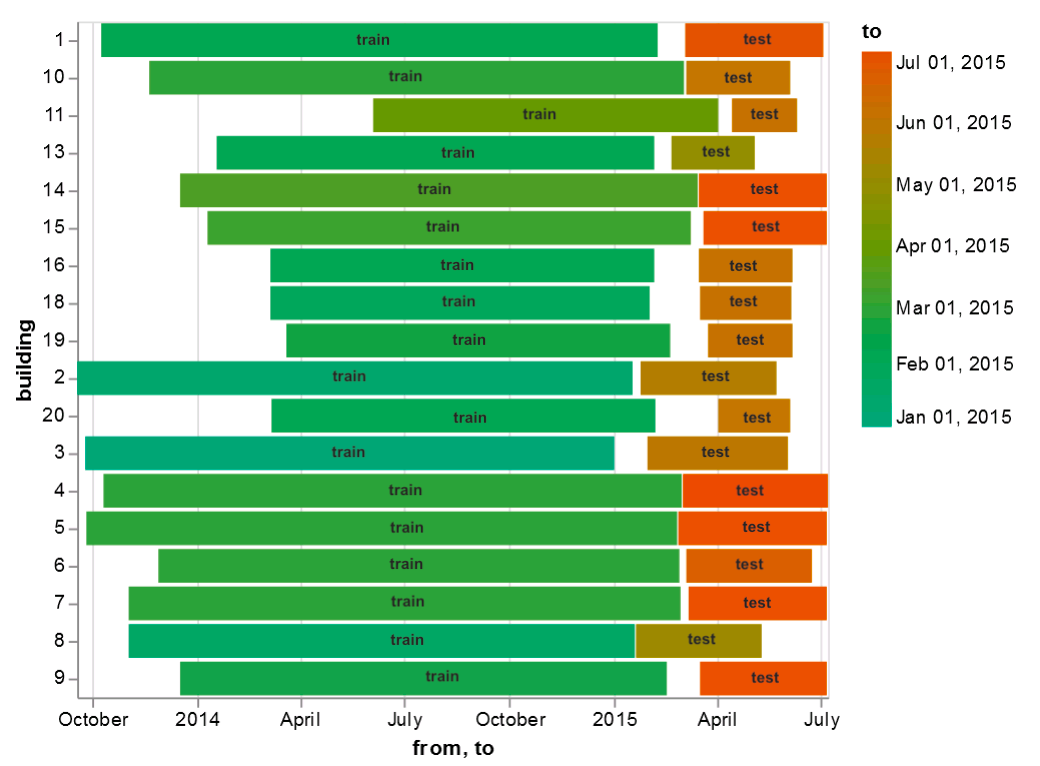
\includegraphics[width=1\textwidth]{Figures/EC/refit_timeline.png}
	\label{fig:refit_timeline}
\end{figure}
fd
\subsubsection{UK-DALE} 

All trough the uk-dale dataset is of similar size, the most of the data is from building 1.
It general it includes 5 years of data, but only for some appliances, with addition there 
are many appliances that are rarely used.
When taking all of this into account, there is to many issues with it and it was simply ignored.
Another issue that can be seen on \ref{fig:ukdale_timeline} is that there is not enough data for 
building 3. Test includes only a week of data, which is not enough for repesentative results, therefore it was ignored.
The rest of the buildings seem healthy.

\begin{figure}[H]
	\centering
	\caption{"Timeline for UK-DALE "}
	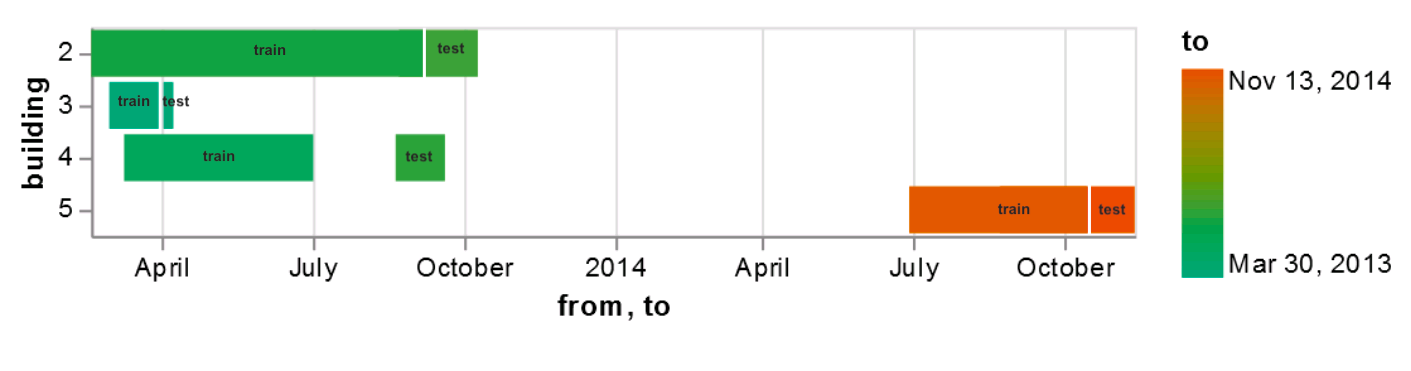
\includegraphics[width=1\textwidth]{Figures/EC/ukdale_timeline.png}
	\label{fig:ukdale_timeline}
\end{figure}

\subsubsection{ECO}
ECO dataset is has decent lengt of data, similar to uk-dale. 
Only issue is building 1, where there is a lot of missing data.
This is a good example how data is split, it is split based on number of samples,
meaning that there is 80 \% in the train bar, due to missing data the second bar is longer. 

\begin{figure}[H]
	\centering
	\caption{"Timeline for ECO"}
	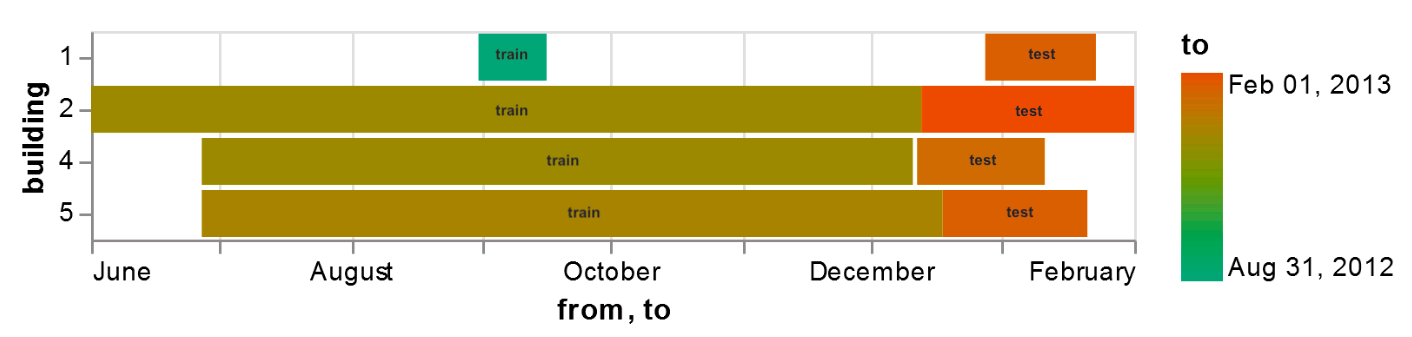
\includegraphics[width=1\textwidth]{Figures/EC/eco_timeline.png}
	\label{fig:eco_timeline}
\end{figure}

\section{Results}

\subsection{The ratio}

Due to lack of ground truth data of actual accidents, it is hard to determine the 
exact accuracy of this algorithm. Every anomaly detected it is no necessarily an 
actual accident, it could be that user decided to lie in bed a bit longer, or decided to not watch 
the TV in the evening.
One metric that we can use to determine how well the algorithm functions is the anomaliy ratio \ref{arr:anom_ratio}.
The reason behind that is, if the routine rate is high it means that it will be easier to detect.

\begin{itemize}
	\item ratio of 1 would mean that for that bucket household has no routine at all.
    \item ratio of .5 would mean that the routine is being "practiced" every second day
    \item ratio of .2 would mean that routine is broken on average every 5 day
    \item ratio of 0 would mean that this household has a routine that is never broken. 
\end{itemize}

When true anomaly occurs such as fall, the dweller, all through he had the same routine for the past year (ratio is 0), would not be able to practice the routine, and the algorithm will be quite sure that tis is actual anoamly.
Therefore, the higher the ratio the less sure we are that an actual anomaly such as fall occurred.
This is a good alternative measurement, that tells us how well this algorithm will perform. 

\subsubsection{Ratio during the week} \label{sssec:ratio_week}

As the behavior of the dwellers changes, so does the accuracy of the algorithm. 
One observation that was made, was that the routine was higher during the week, than during the weekends,
as can be seen on figures bellow. There is also a 

\begin{figure}[H]
	\begin{subfigure}{.5\textwidth}
		% \centering
		\caption{"Building 2"}
		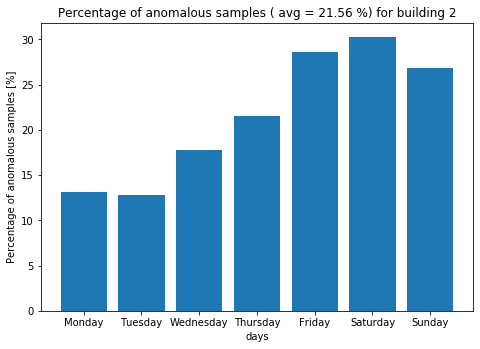
\includegraphics[width=1\linewidth]{../Figures/EC/b2week.png}
		\label{fig:ec_b2week}
	\end{subfigure}%
	~ 
	\begin{subfigure}{.5\textwidth}
		% \centering
		\caption{"Building 19"}
		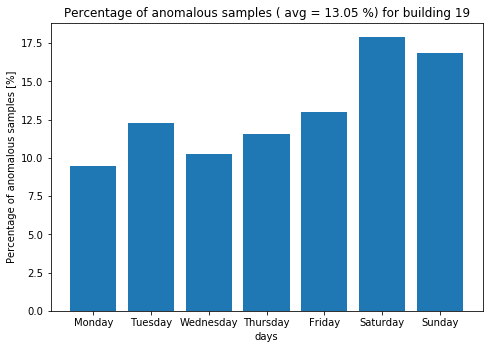
\includegraphics[width=1\linewidth]{../Figures/EC/b19week.png}
		\label{fig:ec_b5week}
	\end{subfigure}%
    \bigskip

    \begin{subfigure}{.5\textwidth}
		% \centering
		\caption{"Building 18"}
		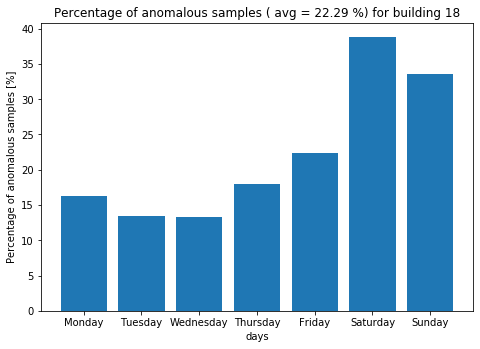
\includegraphics[width=1\linewidth]{../Figures/EC/b18week.png}
		\label{fig:ec_b18week}
	\end{subfigure}%
    ~ 
    \begin{subfigure}{.5\textwidth}
		% \centering
		\caption{"Building 5"}
		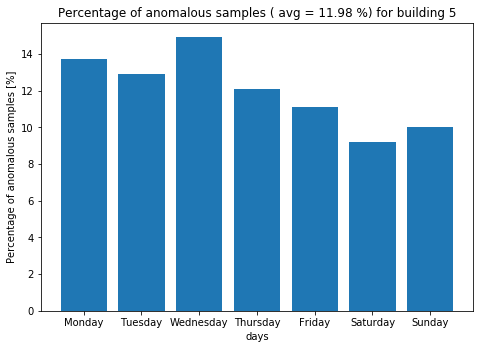
\includegraphics[width=1\linewidth]{../Figures/EC/b5weekd.png}
		\label{fig:ec_b5week}
	\end{subfigure}%
	\label{fig:ec_week}
	\caption{"Weekly anomaly percenage"}
\end{figure}

Since we are dealing with elderly, they have higher routine and their routine does not change that much during the weekends. 
Usualy, asisted living systems are put in place since elders are alone in the dwelling.
Taking all of this into account, we could make an asumption that the routine of elderly is the same trough the week, and simply ignore the weekends. 
This should yield "real/accurate" results. 

\subsection{Ratio in a year}

The ratio also changes over the course of a year. While on average the ratio is lower during the winter, spring and summer, it is higher during the summer due to vacationing. 
This can be seen on figures bellow. 

\begin{figure}[H]
	\begin{subfigure}{.5\textwidth}
		% \centering
		\caption{"Building 2"}
		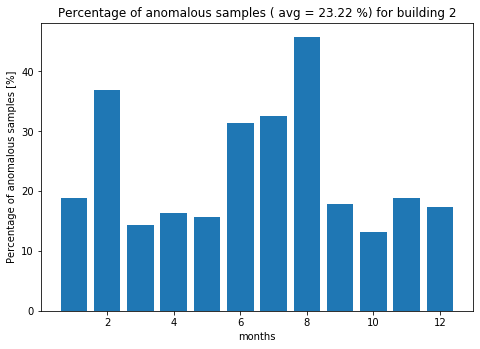
\includegraphics[width=1\linewidth]{../Figures/EC/b2year.png}
		\label{fig:ec_b2year}
	\end{subfigure}%
	~ 
	\begin{subfigure}{.5\textwidth}
		% \centering
		\caption{"Building 19"}
		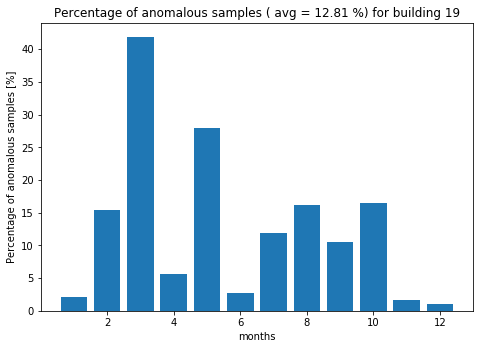
\includegraphics[width=1\linewidth]{../Figures/EC/b19year.png}
		\label{fig:ec_b5year}
	\end{subfigure}%
    \bigskip

    \begin{subfigure}{.5\textwidth}
		% \centering
		\caption{"Building 18"}
		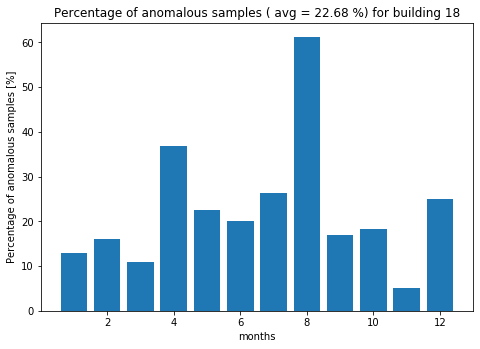
\includegraphics[width=1\linewidth]{../Figures/EC/b18year.png}
		\label{fig:ec_b18year}
	\end{subfigure}%
    ~ 
    \begin{subfigure}{.5\textwidth}
		% \centering
		\caption{"Building 5"}
		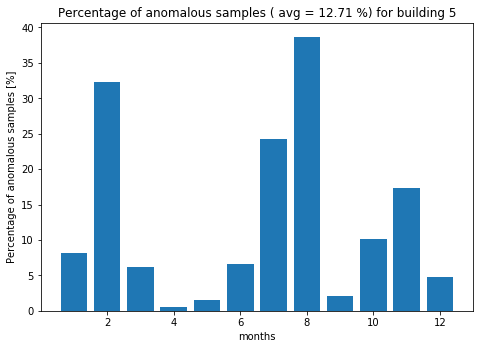
\includegraphics[width=1\linewidth]{../Figures/EC/b5year.png}
		\label{fig:ec_b5year}
	\end{subfigure}%
	\label{fig:ec_year}
	\caption{"Yearly anomaly percentage"}
\end{figure}


The examples above were a demonstration and look into data and metric. 
The examples shown were trained and evaluated on same data. 
In order to show true performance, we will used test data to determine the actual perfomance. 

Results were obtained for 3 datasets. 
REDD and iAWE datasets were not used, since the dataset was to short, they contained less than a month of data. 


\subsection{REFIT}

\subsubsection{Results including weekend data}
results show, that the method in on average 23.6 \% efficient. 
on figure \ref{fig:refit_res} it is possible to see that house 6 yeilds lower results, and house 19 much higher than the rest. 
This could be due to various dataset errors that occured during sampling.

\begin{figure}[H]
	\centering
	\caption{"Results for REFIT "}
	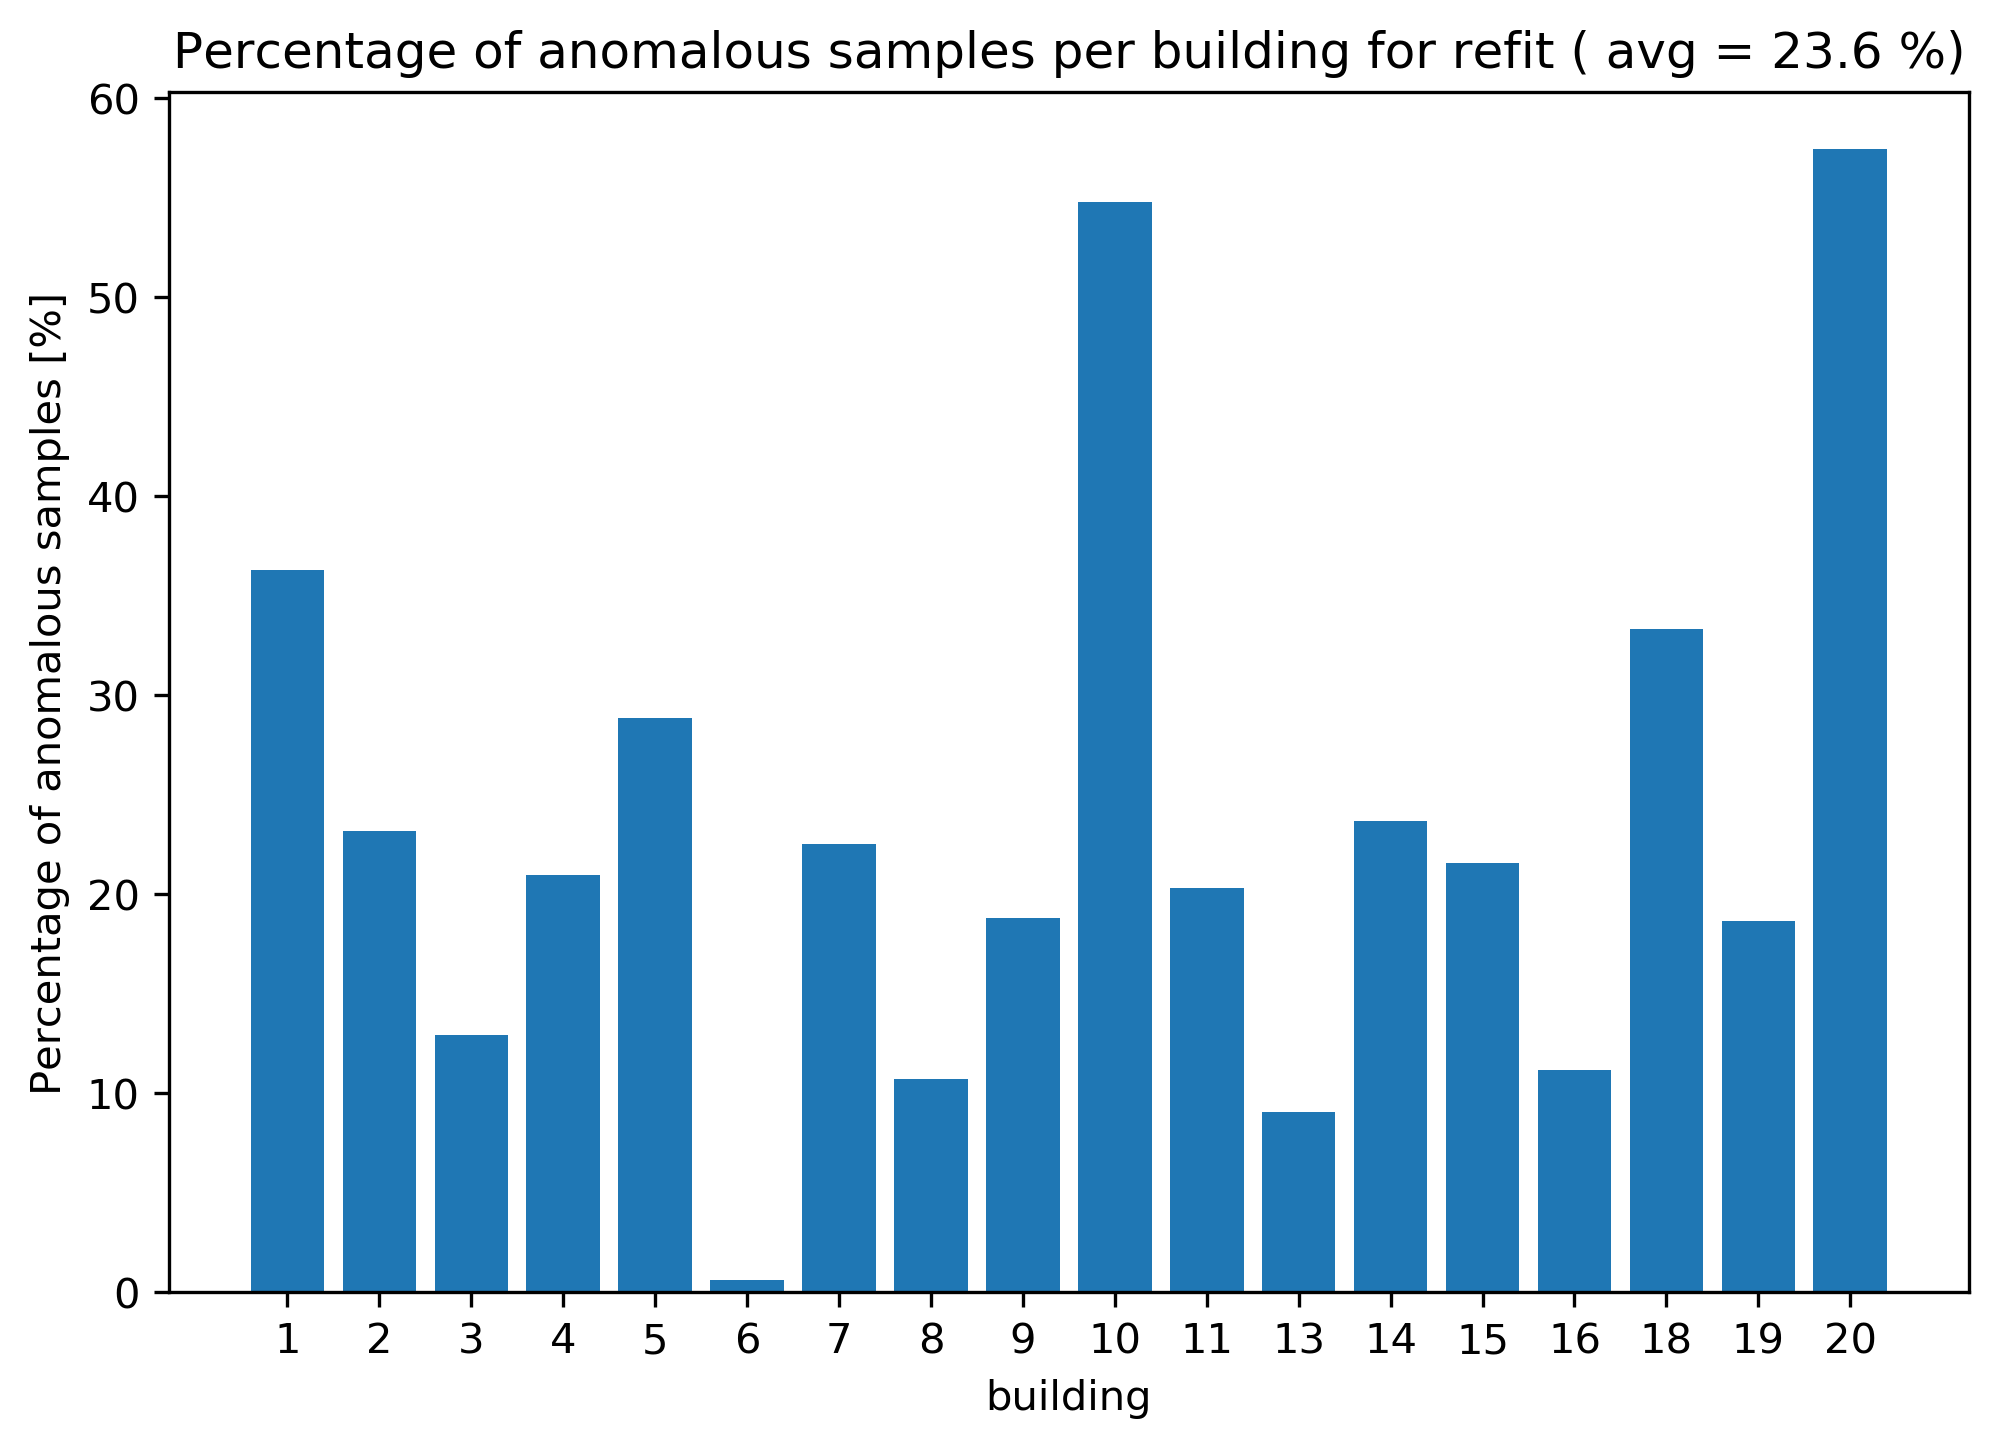
\includegraphics[width=1\textwidth]{Figures/EC/refit_res.png}
	\label{fig:refit_res}
\end{figure}

For more relavant results we can ignore the outliers by removing one max and one min building, such as can be seen on figure \ref{fig:refit_res_2}
This yields result 22.92 \%.
If we were to repeat this proces the result would be 21.33 \%.
Since all outliers are removed, the result converges towards 21 \%, which is the relavant value. 

\begin{figure}[H]
	\centering
	\caption{"Results for REFIT with removed outliers "}
	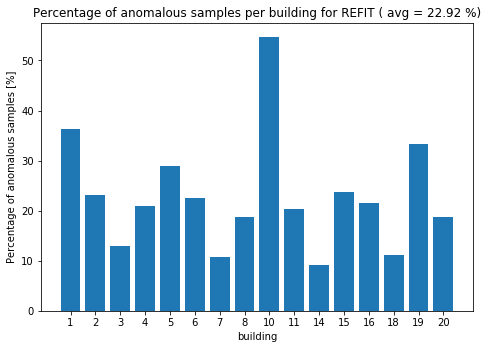
\includegraphics[width=1\textwidth]{Figures/EC/refit_res2.png}
	\label{fig:refit_res2}
\end{figure}

\subsubsection{Results omiting weekend data}

As mentioned in sub-subsection \ref{sssec:ratio_week}, the average routine is different during the week and weekends.
The asumption was that the rutine of elderly people does not change significantly over the week, therefore results should be more relavant if we ignore the weekends.
The results on figure \ref{fig:refit_res_nw_1"} show that result did improve for 1.2 \% to 22.48 \%.

\begin{figure}[H]
	\centering
	\caption{"Results for REFIT weekday only"}
	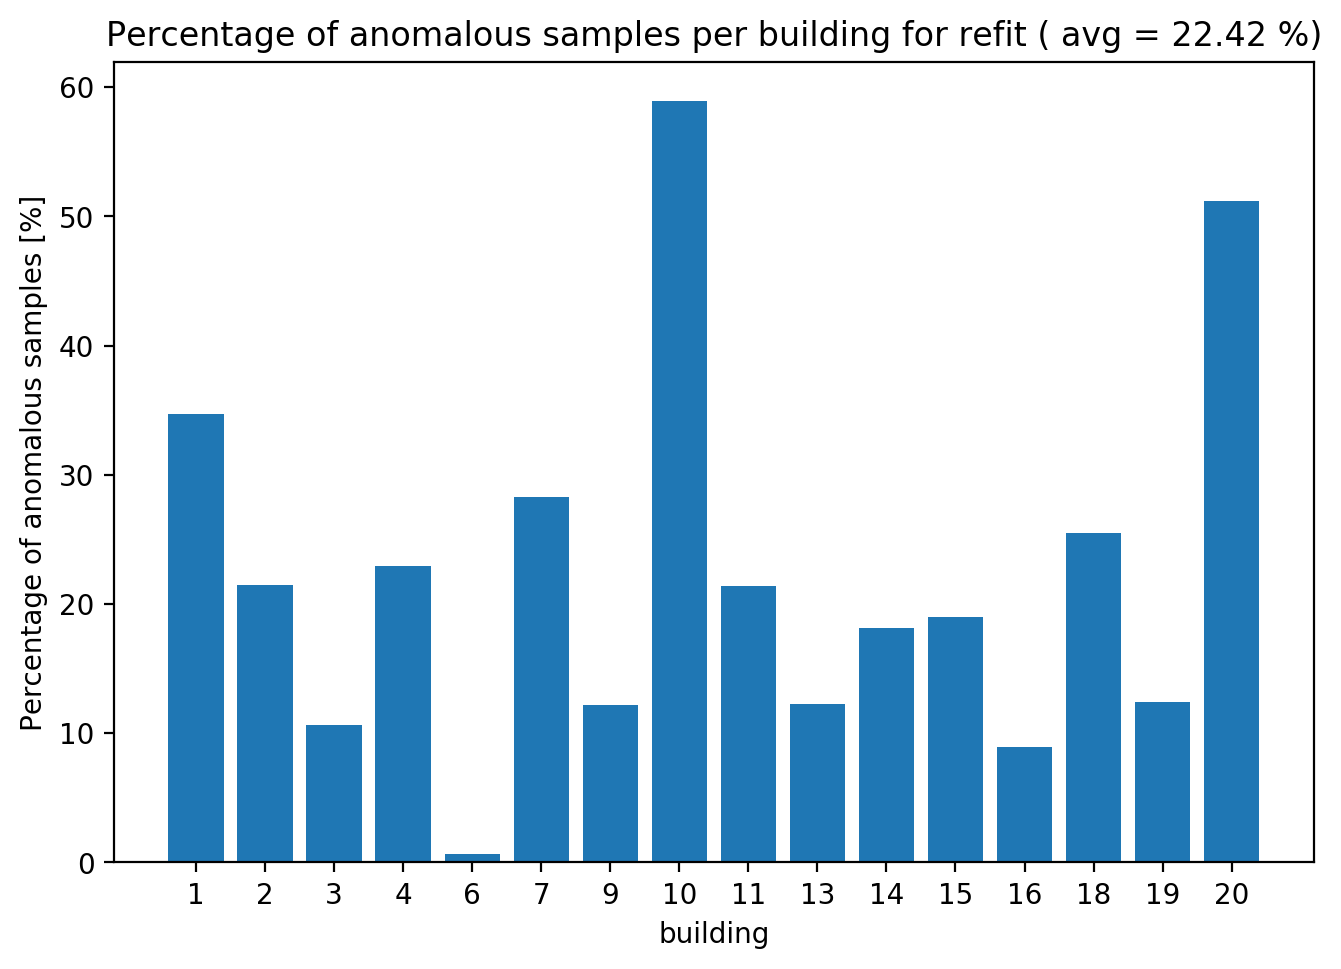
\includegraphics[width=1\textwidth]{Figures/EC/refit_res_nw_1.png}
	\label{fig:refit_res_nw_1"}
\end{figure}

By ignoring the minimal and maximal outliers the results drops to 21.33 \%.
By repeating the process one more time the result drops to 19.91 \%, since all outliers were removed, the result converges towards this value. 

By removing the weekend data, the results decreased for 1.2 \%. 

\begin{figure}[H]
	\centering
	\caption{"Results for REFIT weekday only and removed outliers"}
	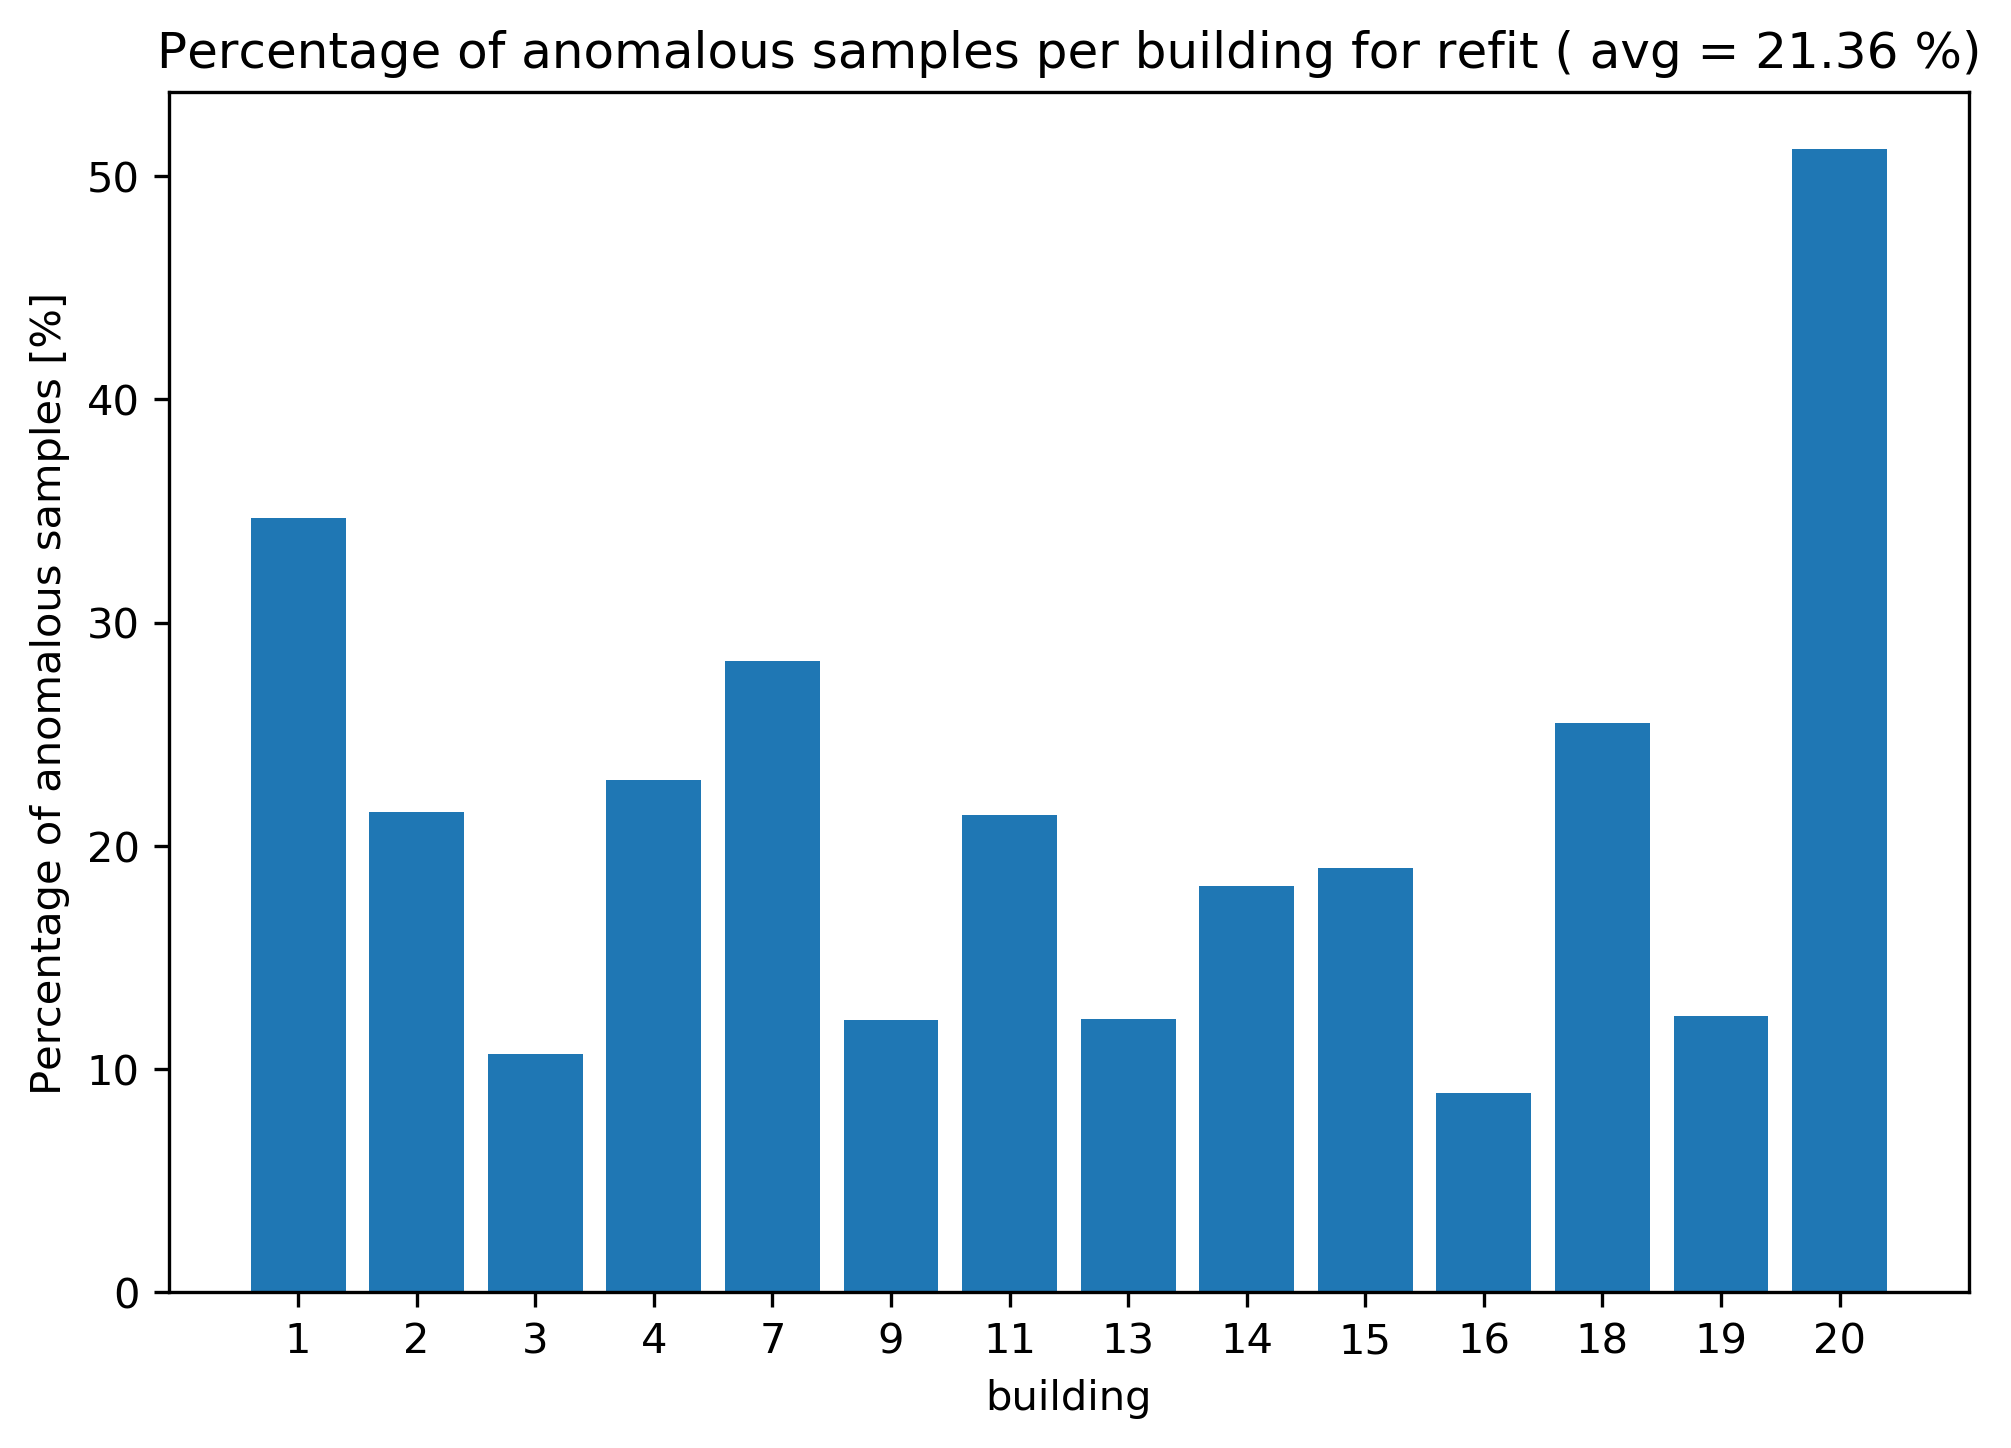
\includegraphics[width=1\textwidth]{Figures/EC/refit_res_nw_2.png}
	\label{fig:refit_res_nw_2"}
\end{figure}

\subsection{UK-DALE}

As mentioned in subsection \ref{ssec:ds_eval}, the ukdale not as long, large and cleaned as the previous dataset, so results could be less relavant.
The results on figure \ref{fig:ukdale_res}, show that the average result is 25.35 \%. Due to low number of buildings, it is not possible to ignore and find outliers. 
\begin{figure}[H]
	\centering
	\caption{"Results for UK-DALE"}
	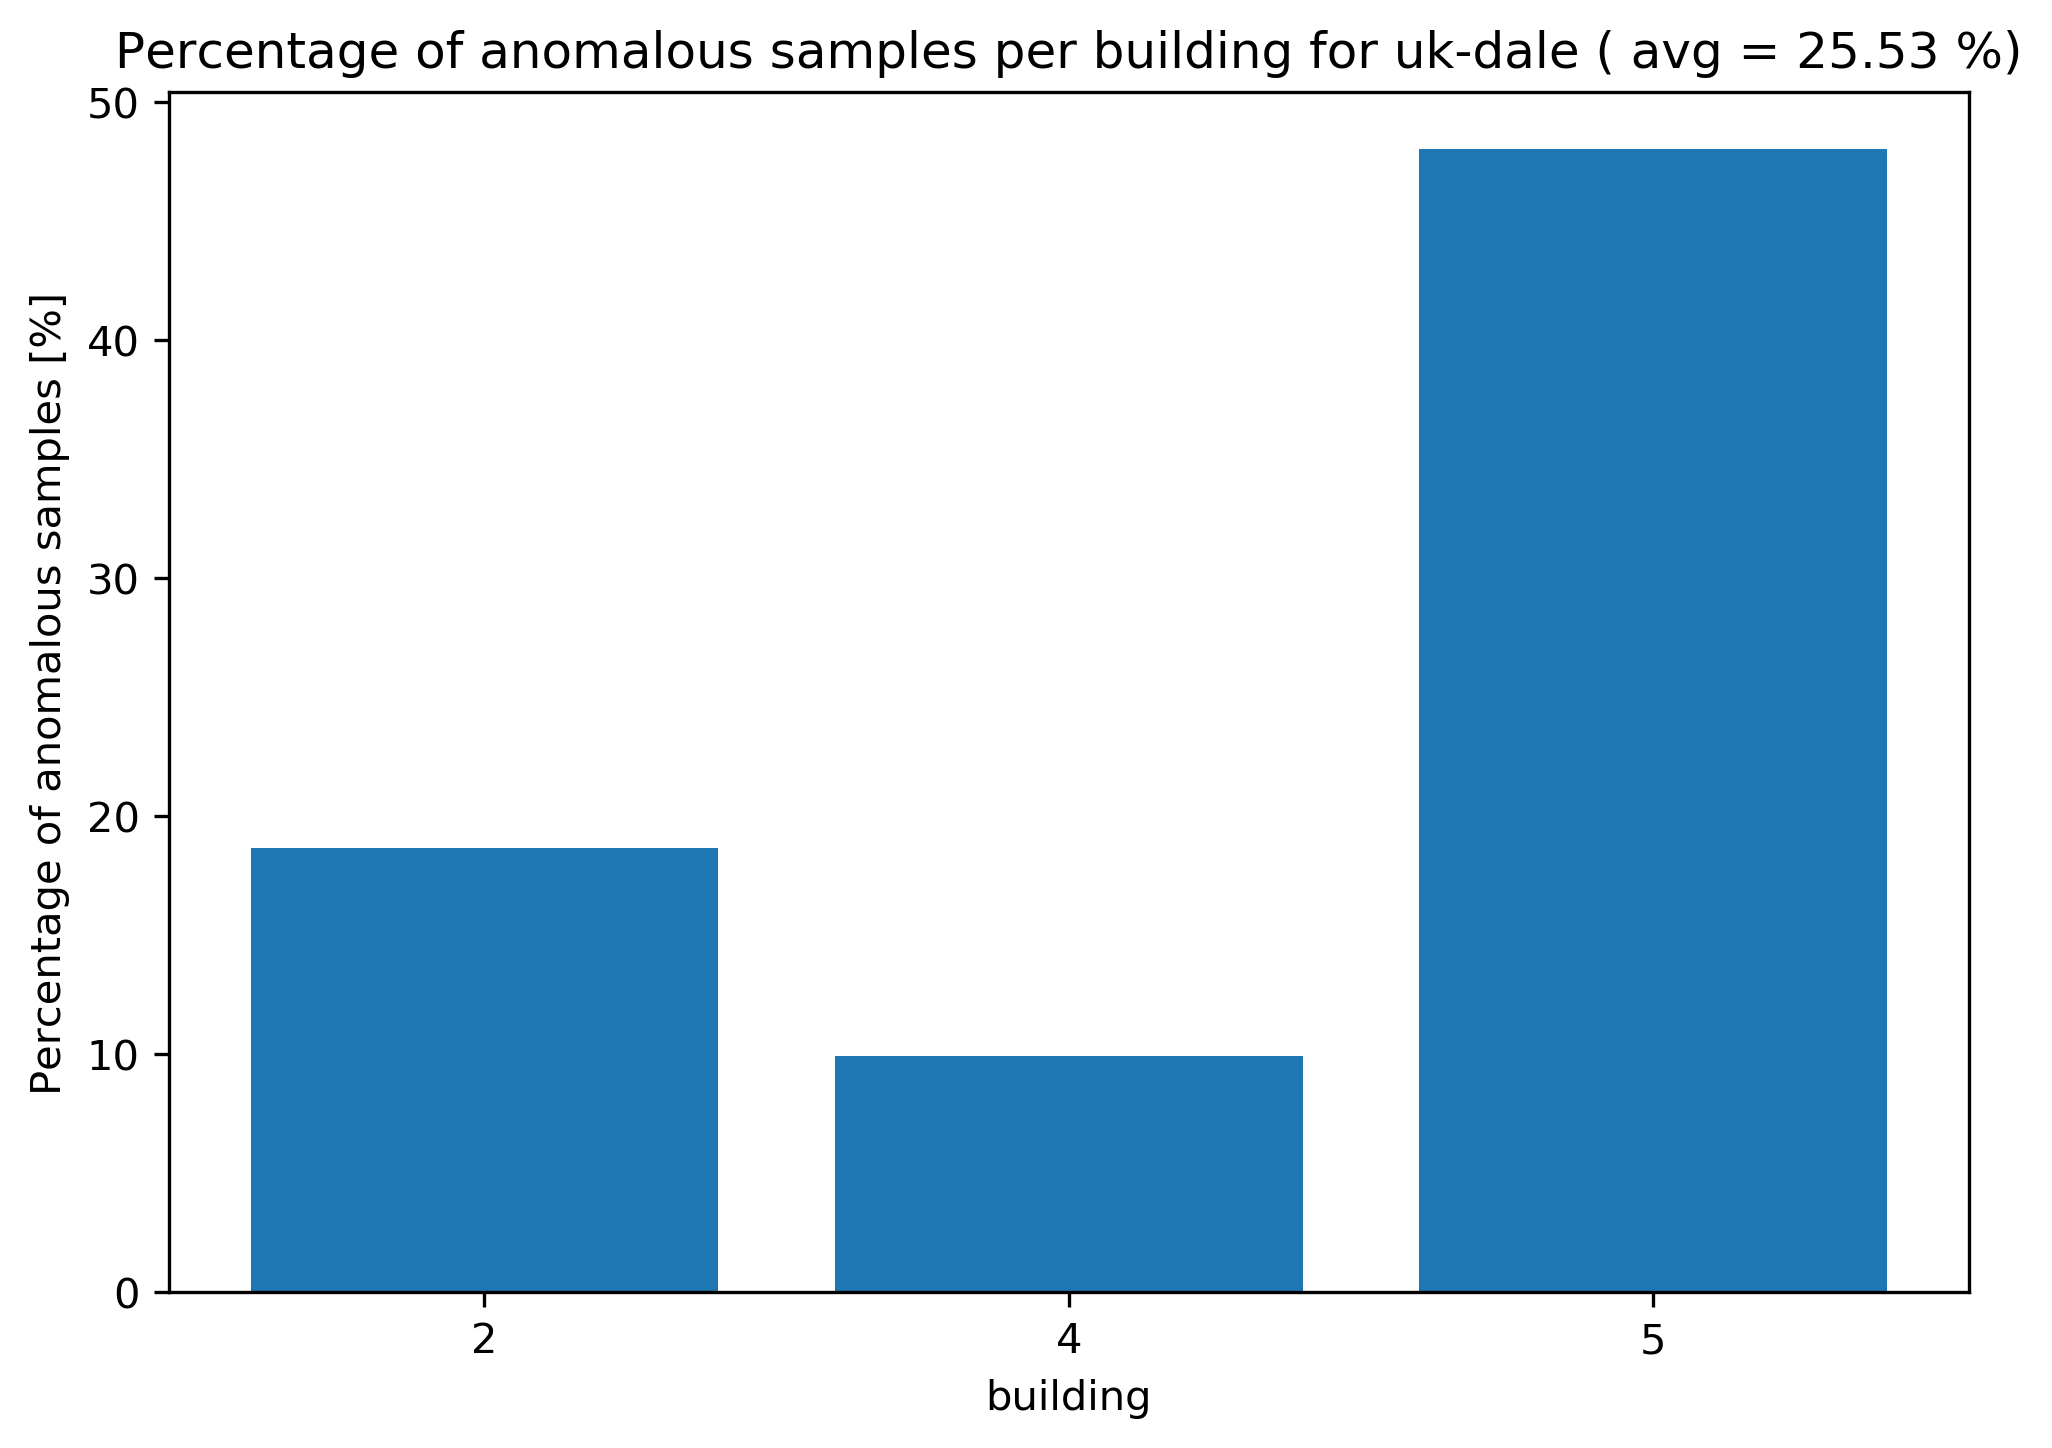
\includegraphics[width=1\textwidth]{Figures/EC/ukdale_res.png}
	\label{fig:ukdale_res}
\end{figure}

The same as for REFIT, the weekend data can be ignored,
In this case, this does not improve the result. 

\begin{figure}[H]
	\centering
	\caption{"Results for UK-DALE omitinng weekends  "}
	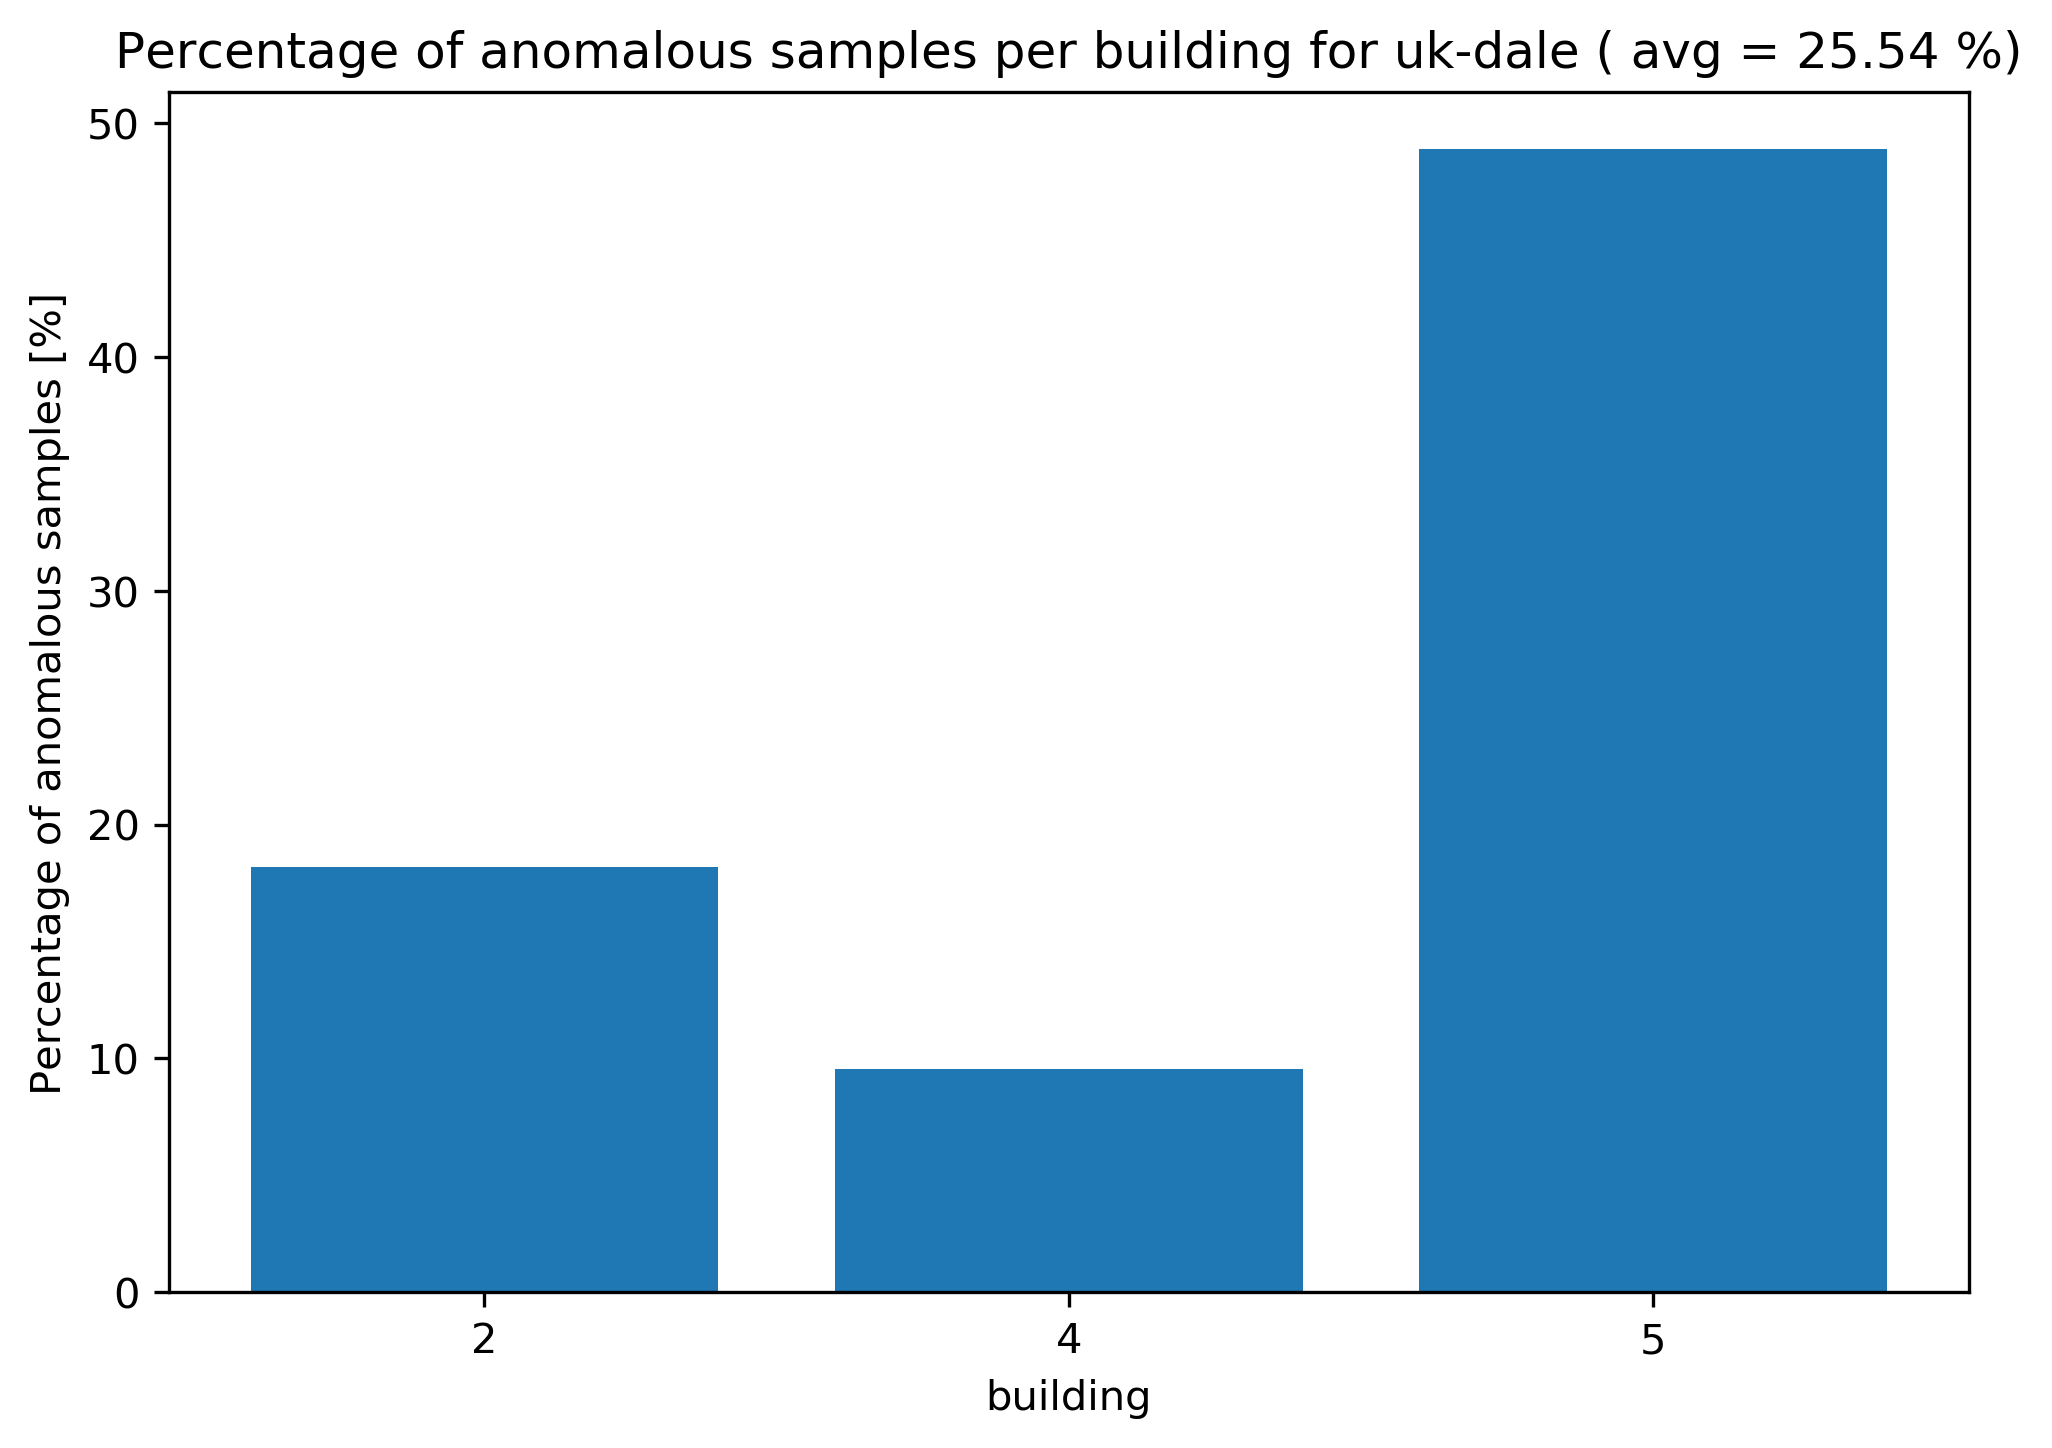
\includegraphics[width=1\textwidth]{Figures/EC/ukdale_nw_res.png}
	\label{fig:ukdale_res_nw}
\end{figure}

\subsection{ECO}

ECO is of the similar quality as UK-DALE as can be seen in \ref{ssec:ds_eval}, regarding the number of buildings and the length of data.
The results \ref{fig:eco_res}, show that this dataset performed the best, with results of 16.32 \%.

\begin{figure}[H]
	\centering
	\caption{"Results for ECO "}
	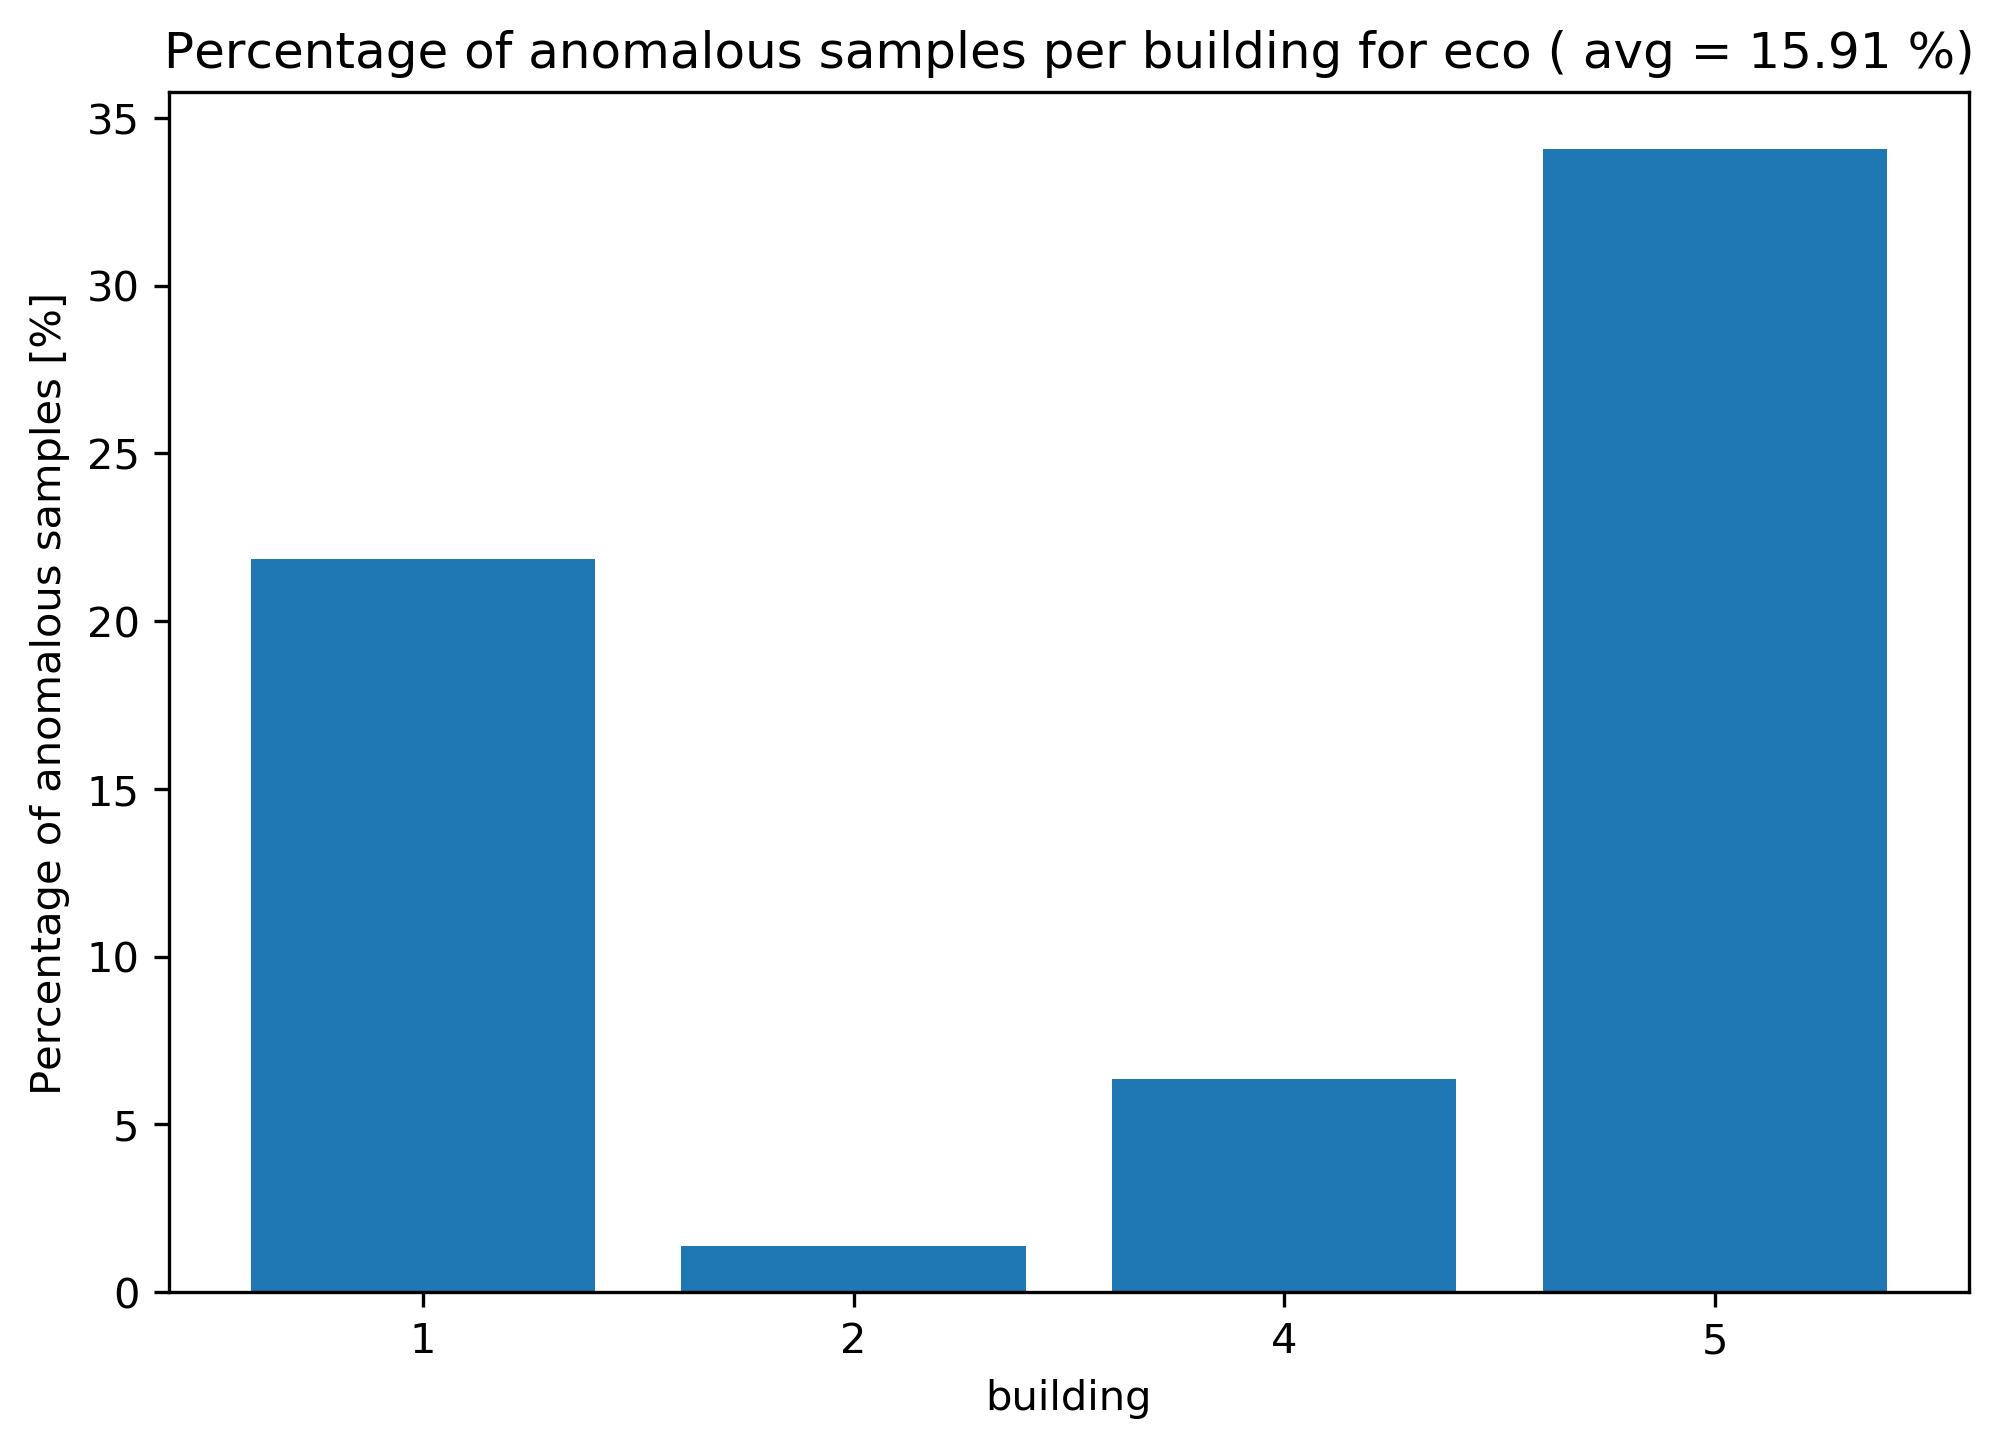
\includegraphics[width=.8\textwidth]{Figures/EC/eco_res_nw_1.png}
	\label{fig:eco_res}
\end{figure}

The same as before we can omit weekend data, which as can be seen on \ref{fig:eco_res_nw} brings the result down to 15.91 \%. 

\begin{figure}[H]
	\centering
	\caption{"Results for ECO omiting weekends "}
	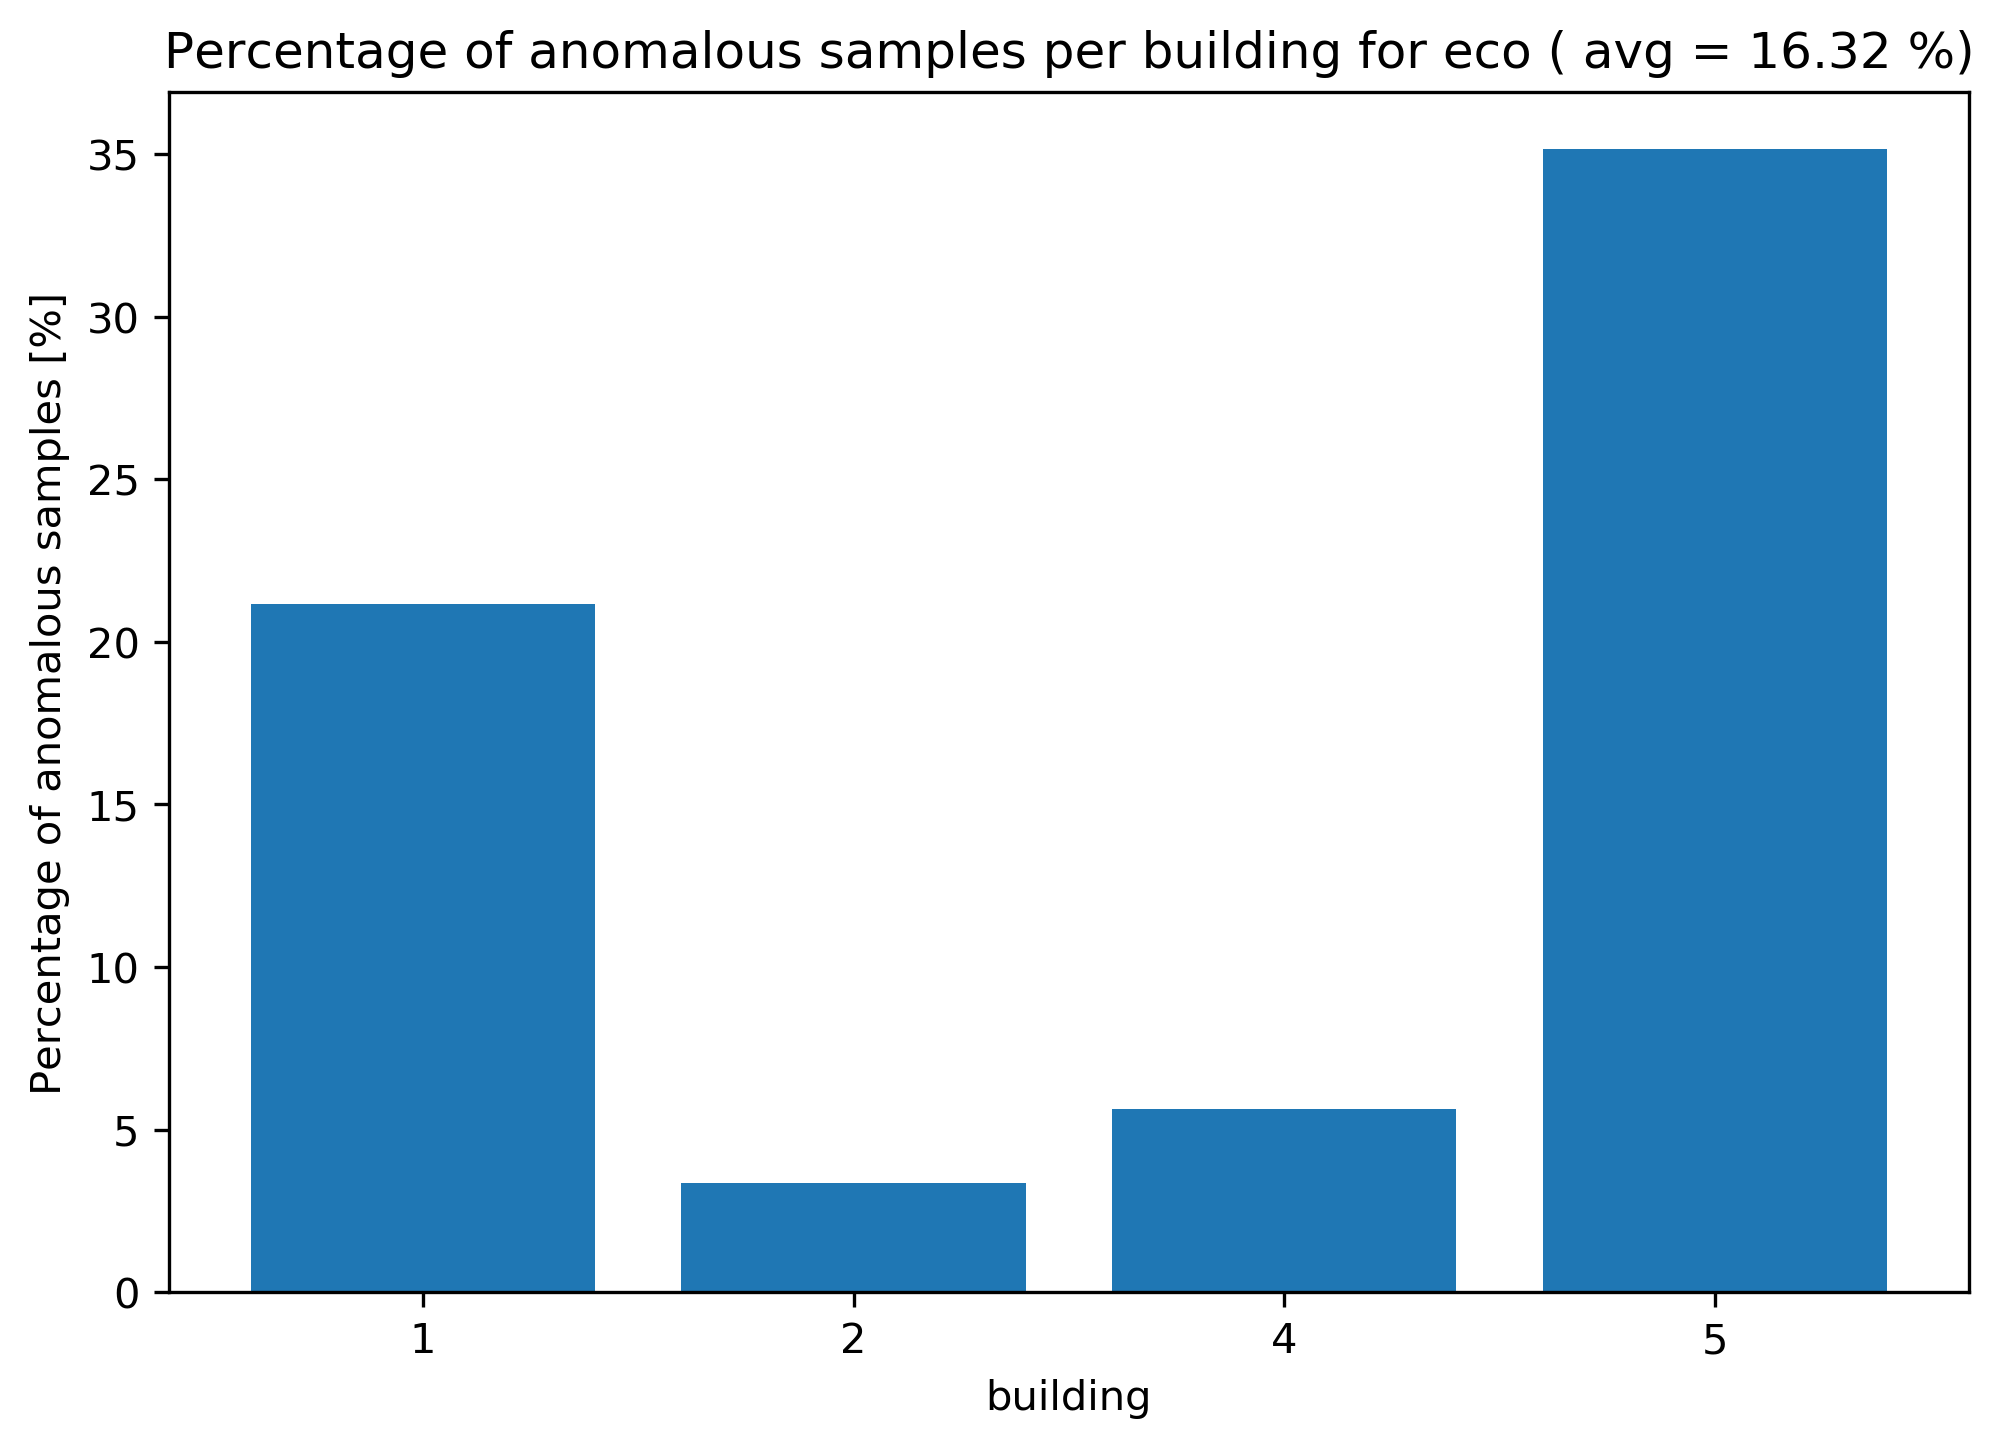
\includegraphics[width=1\textwidth]{Figures/EC/eco_res.png}
	\label{fig:eco_res_nw}
\end{figure}

\subsection{Combined}

After combining results from all 24 buildings, the following table \ref{tab:ec_res} can be populated.
The most relavant results can be seen in the last row.
\begin{table}[H]
    \centering
    \caption{Combined percentage of anomolous samples [\%]}
    \begin{tabular}{|l|ll|ll|}
    \hline
    N = 24 &
      \multicolumn{2}{l|}{\begin{tabular}[c]{@{}l@{}}Including \\ weekend data\end{tabular}} &
      \multicolumn{2}{l|}{\begin{tabular}[c]{@{}l@{}}Excluting \\ weekend data\end{tabular}} \\ \hline
    \begin{tabular}[c]{@{}l@{}}Removed \\ min/max\\ outliers\end{tabular} &
      \multicolumn{1}{l|}{train } &
      test &
      \multicolumn{1}{l|}{train} &
      test \\ \hline
    0 & \multicolumn{1}{l|}{15.92} & 23.71 & \multicolumn{1}{l|}{14.39} & 22.78 \\ \hline
    1 & \multicolumn{1}{l|}{16.05} & 23.19 & \multicolumn{1}{l|}{14.45} & 22.11 \\ \hline
    2 & \multicolumn{1}{l|}{16.02} & 22.62 & \multicolumn{1}{l|}{14.43} & 21.64 \\ \hline
    \end{tabular}
    \label{tab:ec_res}
\end{table}

Results show that the algorithm on average 22 \% of samples will be a false positive, meaning
every 5. sample could be a false positive. In other words the algoritm will be 78 \% efficient at 
detecting true anomalies. 

When analysing these reslts it is good to keep in mind, that this are the results from
various buildings, usualy with more than one user. Elderly are usualy single, or 
a couple, with a higher routines than the rest of population. 